\chapter{The Molecular Docking Problem}
\label{chapter:molecularDocking}
\index{Molecular Docking}

This section has been divided in three subsections. In the Section~\ref{sec:molecularDockingDefinition}, we have defined the molecular docking problem and described the importance of the application of molecular docking approaches in the context of drug discovery. Section~\ref{sec:problemFormulation} included the molecular docking problem formulation for the mono-objective and multi-objective optimizations. Finally, in Section~\ref{sec:reviewStateArt}, we have concluded with a complete review of those studies in which optimization techniques are applied to solve the molecular docking problem.

\section{Molecular docking: Definition and biological significance}
\label{sec:molecularDockingDefinition}

The research based-pharmaceutical industry has increasingly included computational approaches to know the intricate aspect of intermolecular recognition. These approaches have evolved hand-by-hand with biomolecular spectroscopic methods such as the X-ray crystallography and NMR that have an important impact in molecular and structural biology discovery \cite{Ferreira2015}. These experimental techniques have allowed to discover the resolution of more than 100,000 tridimensional structures as the PDB specifies. However, to analyze how the molecules with a known resolution interact, it is necessary to integrate studios \emph{in silico} and experimental techniques.

In the context of structure-based drug design (SBDD) methods, there are three computational techniques which are widely used such as molecular docking, structure-based virtual screening (DBVS) and also molecular dynamics (MD) in order to determine binding energies between a ligand and a given therapeutic target, molecular interactions between atoms and also the changes of molecules' conformations during an interaction. A different approach to the SBDD is the ligand-based structure design (LSBD) which consists of the use of libraries of active ligands and computational approaches (as molecular docking) to detect possible therapeutic targets.

The molecular docking is one of the approaches used in SBDD which tries to predict the conformation of small molecules to a binding site of a given macromolecule that can be a therapeutic target. In the process of SBDD, studies \emph{in silico} like molecular docking are performed to identify candidate ligands to a target. The PDB database currently contains 130,599 biological macromolecules structures which most of them are involved in metabolic and biosignaling and therefore, they can be possible therapeutic targets. Once that the ligand-receptor (the ligand-receptor complex) has been identified in terms of energetic affinity and molecular interactions, the ligand can be modified to increase its efficiency to bind to the therapeutic target. The results are analyzed using molecular docking to know how these molecular modifications alter the binding efficiency of the ligand.

The application of the molecular docking to the SBDD is possible given the accuracy of the ligand-protein predictions performed by molecular docking softwares. The main objective of the molecular docking is to determine the minimal binding energy of the predicted ligand-macromolecule complex. The more negative the obtained binding energy score is, the more stable the ligand-receptor interaction is and thus, the ligand is likely more efficient inhibiting the therapeutic target.

In the computational development of molecular docking software, researchers in this field have traditionally focused on two of the components which determine the quality of the results obtained from the molecular docking software: the energy scoring function and the optimization algorithm. The energy scoring function evaluates the conformation with a given binding energy score. In the literature, there are molecular docking software tools that use different energy scoring functions such as AutoDock \cite{Morris2009}, AutoDock Vina \cite{Trott2010}, GOLD \cite{Verdonk2003} etc. In fact, there have been some studies based on replacing and comparing energy functions in terms of accuracy of ligand affinity predictions and speeding as is reported in \cite{Chang2010}. However, in this dissertation, we have focused on the optimization algorithms by doing an extensive study based on the application of mono- and multi-objective algorithms to solve the molecular docking problem. In the following section, we have introduced the formulation of the problem, how the solutions have been encoded for the mono- and multi-objective optimization approaches and a full description of the objectives that were optimized.

\section{Problem formulation}
\label{sec:problemFormulation}

The main objective of the molecular docking problem is to find an energetically stable complex between a ligand, which can be a small compound (e.g. metabolite, inhibitors etc.), a peptide or a peptidomemetic inhibitor and a macromolecule. There are some computational tools to predict ligand-receptor complexes. In this thesis, we have selected AutoDock 4.2 which is one of the most popular and cited molecular docking software in the research community \cite{Sousa2006,Cosconati2010}. AutoDock 4.2 is a C++ software package that provides an energy scoring function and several algorithms such as an Simulated Annealing (SA) and two Genetic Algorithms (GAs), one of which, referred to as the Lamarckian Genetic Algorithm (LGA), which incorporates a local search \cite{Morris1998}. AutoDock 4.2 energy scoring function is a semi-empirical force field which allows to apply flexibility in ligand and side-chains of protein's aminoacids. The method to apply flexibility in the macromolecule is the same as used in the conformational space of the flexible ligand. The application of flexibility to the ligand and receptor makes the docking simulations more realistic and gives more complexity to the problem increasing the freedom degrees. The limit of freedom degrees that can be applied to AutoDock 4.2 function is 32 \cite{Morris2009}.

For the mono-objective and multi-objective optimization, the solution of the ligand-receptor complex is encoded in the same way. As illustrated in Fig. 3.1, each problem solution for AutoDock 4.2 and jMetal is encoded by a real-value vector of $n$ + 7 variables, in which the first three values correspond to the ligand translation involving the three axis values ($x$, $y$, $z$) in Cartesian coordinate space, the next four values correspond to the ligand and/or macromolecule orientation, and the remaining n values are the ligand and macromolecule torsion dihedral angles. For the mono- and multi-objective approaches, we have used a grid-based methodology provided by AutoDock in which the macromolecule's interaction site is embedded in a 3D rectangular grid. For each point of the grid, the electrostatic interaction energy and the van der Waals terms for each ligand atom type are pre-computed and stored, taking into account all the protein atoms. In this way, the protein contribution at any given point is obtained by tri-linear interpolation in each grid cell. This interpolation leads to a range of translation variables ($x$, $y$, $z$) of 120 grid spacing points dimension \cite{web-autodock}. The values of these variables are delimited between the range of the coordinates of the grid space that has been chosen for each problem. All ranges are selected randomly, so if the center of the grid is for example the (10, 10, 10) point, a solution with values of ten in its $x$, $y$ and $z$ will be in such a position. In the case of orientation (quaternion) and torsion variables, they are measured in radians and encoded in the range of [-$\pi$, $\pi$].

\begin{figure}[H] %tb
\vspace{0.5cm} \centering 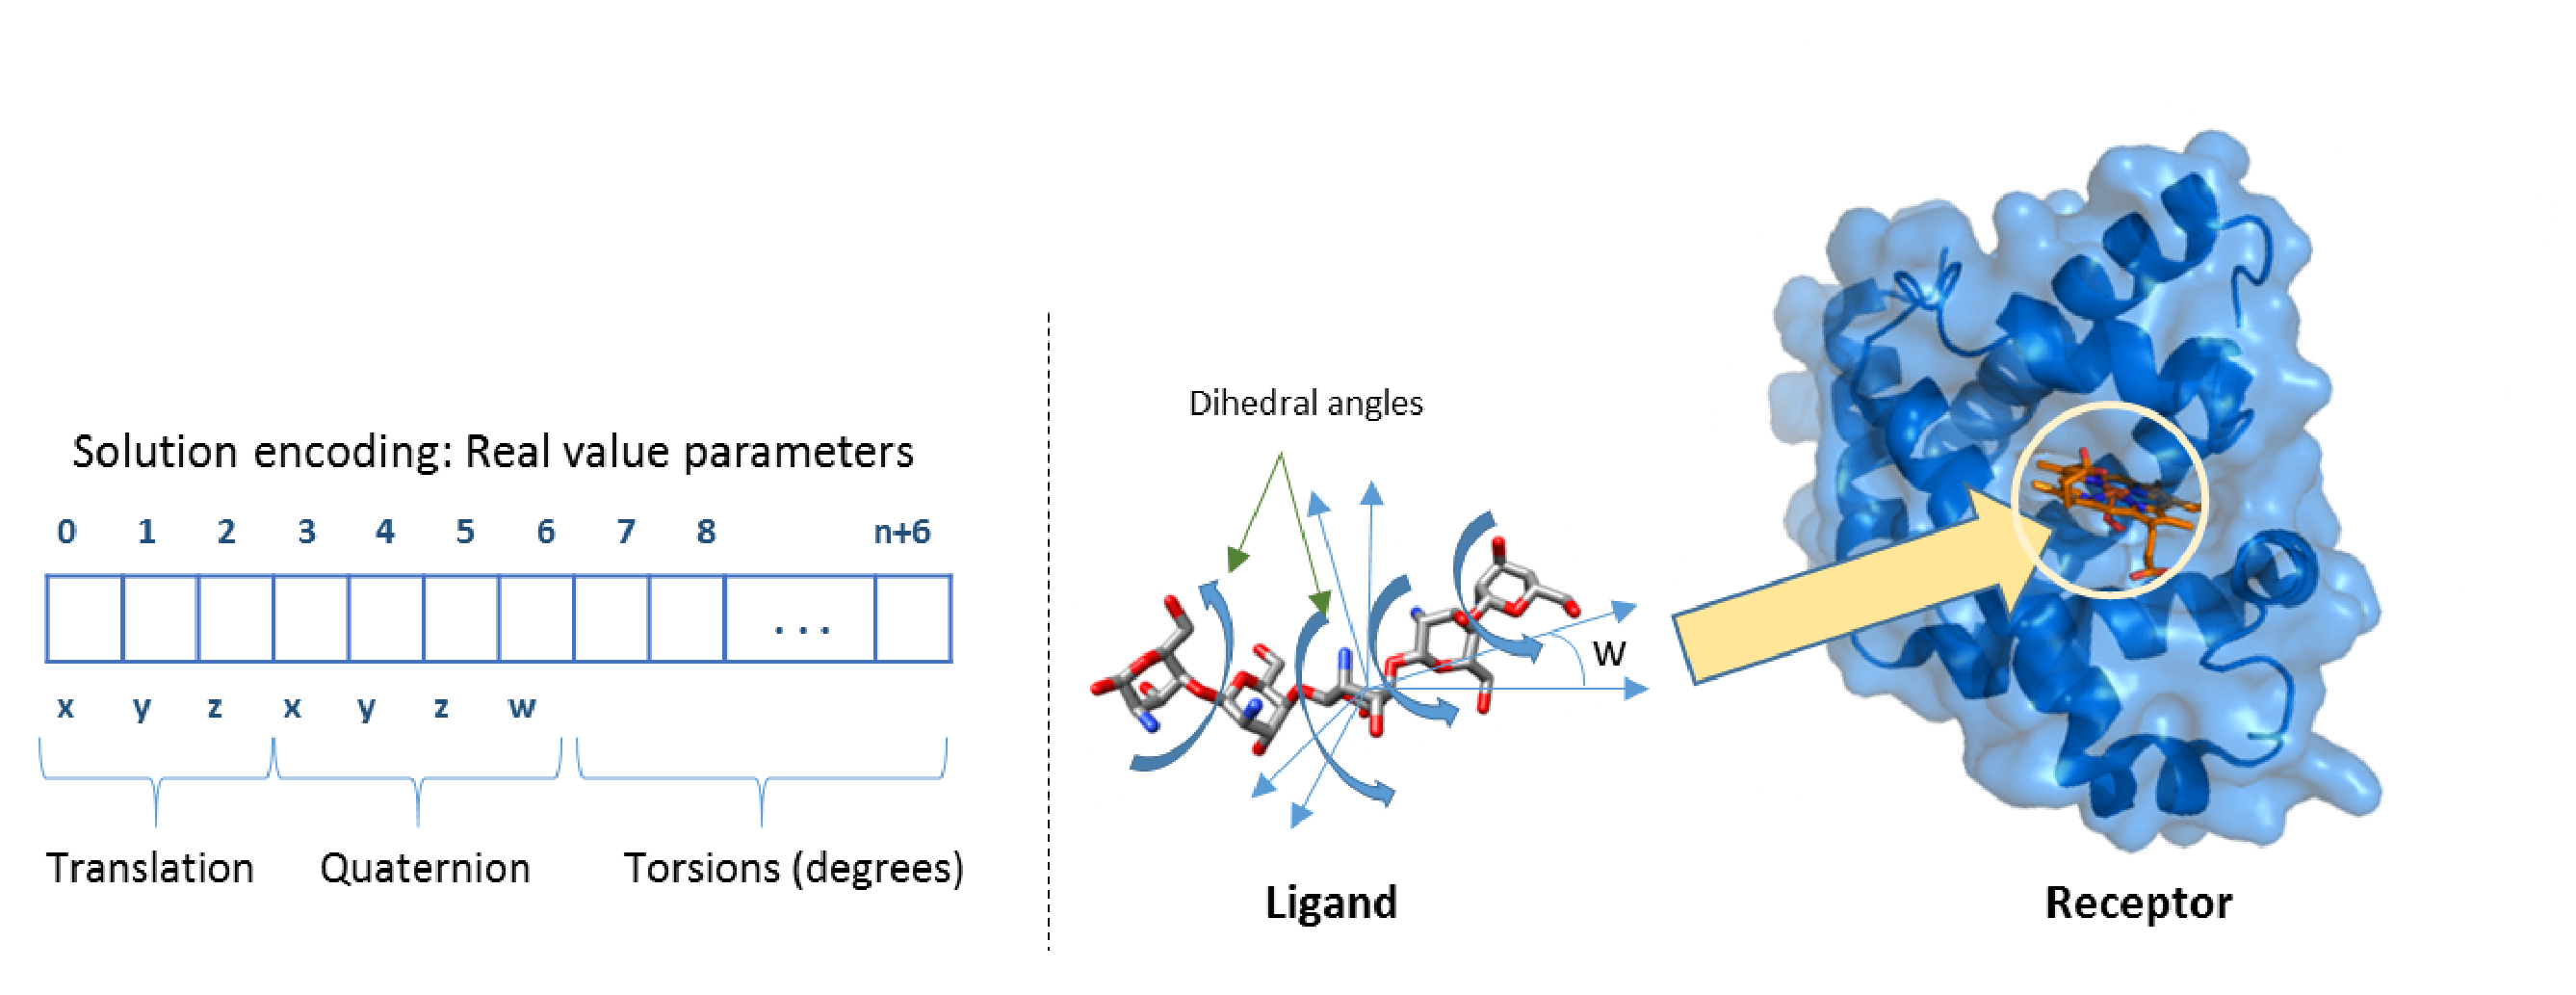
\psfig{file=./img/dockingProblem/encoding.eps,width=\textwidth}
\caption[Solution encoding in AutoDock 4.2 and jMetal.]{Solution encoding in AutoDock 4.2 and jMetal. The first three values (translation) are the coordinates of the center of rotation of the ligand. The next four values (quaternion) are the unit vector describing the direction of rigid body rotation (x, y and z) and the rotation of the angle degrees (w) that are applied. The rest of the values hold the torsion angles in degrees, being n the number of torsions of the ligand.}\label{img.docking.fig:solution} \vspace{0.6cm}
\end{figure}

\subsection{Mono-objective optimization}
\label{subsection:mono_solution}

In the mono-objective optimization approach, the objective to optimize is the final free binding energy ($\Delta$G), which is measured in kcal/mol. The more negative $\Delta$G is, the more stable the computed ligand-receptor complex. $\Delta$G is computed by the energy scoring function provided by AutoDock 4.2, which is used to measure the quality of the ligand-receptor binding solutions \cite{Morris2009}. $\Delta$G is calculated according to the following equations (each term of the equations is described below):

\begin{equation}
\label{eq:equation-docking-mono-1}
\begin{split}
\Delta G = (Q_{bound}^{R-L} - Q_{unbound}^{R-L} + \Delta S_{conf}) + (Q_{bound}^{L-L} - Q_{unbound}^{L-L}) + (Q_{bound}^{R-R} - Q_{unbound}^{R-R}) 
\end{split}
\end{equation}

\begin{equation}
\label{eq:equation-docking-mono-2}
\begin{split}
Q = W_{vdw} \sum_{i,j} (\frac{A_{ij}}{r_{ij}^{12}} - \frac{B_{ij}}{r_{ij}^{6}}) + W_{hbond} \sum_{i,j} E(t) \left( \frac{C_{ij}}{r_{ij}^{12}} - \frac{D_{ij}}{r_{ij}^{10}} \right) + \\
+ W_{elec} \sum_{i,j} \frac{q_i q_j}{\varepsilon(r_{ij})r_{ij}} + W_{sol}\sum_{i,j}(S_i V_j + S_j V_i)e^{(-r_{ij}^2/2\sigma^2)}
\end{split}
\end{equation}

\begin{equation}
\label{eq:equation-docking-mono-3}
\begin{split}
\Delta S_{conf} = W_{conf} \cdot N_{tors}
\end{split}
\end{equation}

As formulated in Eq.~\ref{eq:equation-docking-mono-1}, the free binding energy function is calculated
from the differences between ligand/s (L) and receptor/s (R) in bounded and unbounded states. That is, the free energy of binding is based on the evaluation of the transition of the ligand and protein intramolecular energetics from an unbounded to a bounded state, and the intermolecular energetics of ligand–protein complex. Therefore, the force field involves six pair-wise evaluations (V) plus
a term of conformational entropy (Ntors), which is directly proportional
to the number of rotatable bonds of the ligand molecule ( see Eq.~\ref{eq:equation-docking-mono-3}). Each pair of energetic evaluation terms includes the evaluations of dispersion/repulsion (vdw), hydrogen bonds (hbond), electrostatics (elec), and desolvation (sol). Weights $W_{vdw}$, $W_{hbond}$, $W_{conf}$, $W_{elec}$, and $W_{sol}$ of Eqs.~\ref{eq:equation-docking-mono-2} and \ref{eq:equation-docking-mono-3}, are constants for van der Waals, hydrogen bonds, torsional forces, electrostatic interactions, and desolvation, respectively. In Eq.~\ref{eq:equation-docking-mono-2}, $r_{ij}$ represents the interatomic distance, $A_{ij}$ and $B_{ij}$ in the first term are Lennard–Jones parameters taken from Amber force field \cite{Weiner1984}. Similarly, $C_{ij}$ and $D_{ij}$ in the second term are Lennard-Jones parameters for maximum well depth of potential energies between two atoms, and E(t) represents the angle-dependent directionality. The third term in Eq.~\ref{eq:equation-docking-mono-2} uses a Coulomb approach for electrostatics. Finally, the fourth term is calculated from the volume ($V$) of the atoms that are surrounding a given atom weighted by $S$, and an exponential term which involves atom distances.

Ligand–protein docking is a highly complex optimization problem, with unknown optimum and usually characterized by multimodal landscape energy functions \cite{problem-characterization1999}. In addition, the computational cost of each energy evaluation increases with the number of atoms in complex ligand-protein (with thousands of them), hence involving millions of energy evaluations, since a minimum quality of molecular binding is mandatory in molecular docking modeling. Therefore, the use of metaheuristic approaches is highly recommendable for molecular docking, since they are able to explore a great number of combinations with a fast convergence to successful solutions \cite{Blum2011}.

\subsection{Multi-objective optimization}
\label{subsection:multi_solution}

A multi-objective optimization problem is characterized by two spaces: the decision space and the objective space. The former refers to all the possible feasible solutions, and the latter includes their corresponding objective values. 

\textbf{Decision Space}: As mentioned in Section~\ref{sec:problemFormulation}, the AutoDock 4.2 solution for the multi-objective approach is encoded in the same way as the mono-objective approach. This means that all the returned solutions are encoded in a real-value vector of $7 + n$ variables in which the first three values correspond to the ligand translation, the next four values correspond to the ligand and/or macromolecule orientation, and the remaining $n$ values are the ligand and macromolecule torsion dihedral angles. These solutions correspond to the decision space that characterized the multi-objective optimization. It is worth noting that we have also applied the grid-based methodology to define the ligand-receptor binding site.

\textbf{Objective Space}: We have applied two bi-objective formulations. In the first formulation, we have optimized the intermolecular energy ($E_{inter}$) and the intramolecular energy ($E_{intra}$). The values of these terms are given from the AutoDock energy function \cite{Morris2009} (see Eq.~\ref{eq:equation-docking-multi-1}), being opposite between them \cite{Janson2008}, and therefore giving rise to a multi-objective approach of this problem as follows:

\begin{itemize}
\item \textbf{Objective 1}: the $E_{inter}$ energy (see Eq.~\ref{eq:equation-docking-multi-2}) is estimated by the difference of the bound and unbound states of the ligand-macromolecule complex. The $E_{inter}$ energy describes the binding affinity of the conformation. 
\item \textbf{Objective 2}: The $E_{intra}$ energy (see Eq.~\ref{eq:equation-docking-multi-3}) of the ligand and receptor is estimated by the difference between the bound and unbound states of the ligand and receptor. The $E_{intra}$ characterizes the stability of the ligand in terms of energy.
\end{itemize}

\begin{equation}
\label{eq:equation-docking-multi-1}
\begin{split}
\Delta G = E_{inter} + E_{intra} + \Delta S_{conf}
\end{split}
\end{equation}

\begin{equation}
\label{eq:equation-docking-multi-2}
\begin{split}
E_{inter} = (Q_{bound}^{R-L} - Q_{unbound}^{R-L})
\end{split}
\end{equation}

\begin{equation}
\label{eq:equation-docking-multi-3}
\begin{split}
E_{intra} = (Q_{bound}^{L-L} - Q_{unbound}^{L-L}) + (Q_{bound}^{R-R} - Q_{unbound}^{R-R}) 
\end{split}
\end{equation}

For Eq.~\ref{eq:equation-docking-multi-2} and Eq.~\ref{eq:equation-docking-multi-3}, each pair of energetic evaluations terms are described in Eq.~\ref{eq:equation-docking-multi-2} in  subsection \ref{subsection:mono_solution}. The $\Delta S_{conf}$ term is described in Eq.~\ref{eq:equation-docking-mono-2}.

In the second multi-objective formulation, we have optimized the intermolecular energy ($E_{inter}$) and the RMSD score. These two measures are contrary and consequently a bi-objective optimization approach is reasonable with these measures. These objectives are calculated by the following equations:

\begin{itemize}
\item \textbf{Objective 1}: the $E_{inter}$ energy (see Eq.~\ref{eq:equation-docking-multi-2}) of the ligand and receptor is estimated by the difference between the bound and unbound states of the ligand and receptor. The $E_{inter}$ energy describes the binding affinity of the conformation.

\item \textbf{Objective 2}: The RMSD is a measure of distance between the co-crystallized ligand in the receptor and the predicted position of the docking ligand (see Eq.~\ref{eq:equation-docking-rmsd}). The RMSD score is a measure to compare the accuracy of the results obtained from the computational docking approaches. The RMSD takes into account symmetry, partial symmetry (e.g. symmetry within a rotatable branch) and near-symmetry in a simple heuristic way \cite{Trott2010}. The lower the RMSD score, the better the docking solution is. The RMSD cutoff of 2\AA\ is widely considered as a criterion to consider the computed ligand–protein conformation as a good prediction among the research community. This measure is very useful in those cases in which the ligand pose to the macromolecule is known. It is worth mentioning that, from a pharmacological point of view, a ligand conformation with an RMSD score of 0\AA\ (the co-crystallized and computed ligands completely overlap) is not the best solution as the macromolecule could involve other ligand binding sites, which have not been discovered yet.

\end{itemize}

\begin{equation}
\label{eq:equation-docking-rmsd}
\begin{split}
RMSD_{ab} = max(RMSD_{ab}^{'}, RMSD_{ba}^{'}), \; with \; RMSD_{ab}^{'} = \sqrt[]{\frac{1}{N}\sum_{i} \mathop{min}_{\textbf{j}} r_{2}^{ij}}
\end{split}
\end{equation}

The sum is over all $N$ heavy atoms in structure $a$, the minimum is over all atoms in structure $a$ with the same element type as atom $i$ in structure $b$.

\section{Review of the State-of-the-Art}
\label{sec:reviewStateArt}

Over the last two decades, different metaheuristics have been applied as search methods to solve the docking problem \cite{Lameijer2005}. One example is the docking software AutoDock, which incorporates three metaheuristic techniques. AutoDock is considered to be the most cited and one of the most used software packages in molecular modeling studies to discovery new compounds \cite{Sousa2006} as is reported in \cite{Cosconati2010}.

AutoDock was released in 1990, and it included a rapid search method using Monte Carlo simulated annealing \cite{Goodsell1990}. However, this method proved to be inadequate for ligands with more than eight rotatable bonds \cite{Morris1998}. Eight years later, in an attempt to improve the software, AutoDock 3.0 was released, adding the Genetic Algorithm (GA) and the Lamarckian Genetic Algorithm (LGA), which incorporates a local search, and an empirical binding free energy force that enables the prediction of the free binding energies. Docking analyses have demonstrated that the LGA is the most efficient search method of the three AutoDock algorithms in terms of the lowest energy found in a number of energy function evaluations \cite{Morris1998}. AutoDock 4 was presented in 2009 \cite{Morris2009}. It allows conformational models of side chains of proteins, provides torsional degrees of freedom and tries to solve the problem of flexibility in the receptor, a challenge in docking approaches as we have mentioned in section \ref{sec:problemFormulation}. More recently, a new release has appeared, AutoDock 4.2, which incorporates several enhancements over AutoDock 4. The latest version includes a default unbounded state, different to the extended unbounded state of AutoDock 4, an improvement over the time required to run a high-quality docking with flexible and rigid components, involving an attempt to ensure compatibility between the different releases of AutoDock software.

In 2010, as an improvement on the previous releases, the AutoDock authors implemented a new program for molecular docking called AutoDock Vina \cite{Trott2010}. A study performed by Chang \emph{et al.} \cite{Chan2007} compares the two softwares in drug virtual screening being AutoDock and AutoDock Vina very accurate for virtual screening in cases in which ligands had fewer than eight rotatable bonds. The results shown that AutoDock Vina was faster than other molecular docking tools. This can be explained by the improvements implemented in AutoDock Vina such as multithreading to speed up the execution in multicore processors, and the use of an iterated local search algorithm (ILS) as the search engine. The stopping condition of the ILS is adaptively determined, thus making it difficult to compare it fairly with other techniques that use a fixed number of function evaluations.

A number of approaches can be found in the current literature that have proposed metaheuristic techniques designed around AutoDock versions. Atilgan \emph{et al.} \cite{Atilgan2010} developed a new program named AutoDockX which incorporates a sustainable GA, namely Age-Layered Population Structure (ALPS), including the age attribute for individuals. Chen \emph{et al.} \cite{Chen2007} presented an algorithm called SODOCK, which is an adaptation of PSO including Solis and Wets local search and uses an older version of the AutoDock energy function (version 3.05). Two other PSO related proposals are the varCPSO-ls algorithm, an extension of the CPSO algorithm with a local optimizer which is embedded inside the AutoDock 3 source code and uses its energy function \cite{Namasivayam2007}, and the FIPSDock algorithm, which adopts the AutoDock 4.2 energy function \cite{Liu2012}. DE has also been applied in this context. A first attempt is DockDE \cite{Thomsen2003DE}, a variant of DE which uses an older version of the AutoDock energy function. ODE is also an extension of DE enhanced by a local search algorithm and a pseudo-elitism operator, and using the AutoDock scoring function \cite{Koohi-Moghadam2012}. A more recent version is SADock \cite{HwanWon2013}, that incorporates a Hooke Jeeves local search.

Among studies on molecular docking with metaheuristics not based on AutoDock, there are several approaches that are also worth mentioning. PARADockS is a framework implemented to predict the ligand–protein interaction adapting PSO to several objective functions \cite{Meier2010}. An Ant Colony Optimization (ACO) approach is also presented in \cite{Korb2006} using a systematic molecular simulator. A variant of DE called MolDock was parallelized on both GPU and CPU using a fitness function designed by the authors \cite{Simonsen2011}. However, although the technique is adapted to a flexible docking receptor, it has not been evaluated using flexible targets. Other optimization methods such as multi-scale optimization models and information entropy-based searching techniques with narrowing space were applied in a new docking algorithm \cite{Kang2012}. Herberlé \emph{et al.} \cite{Herberle2010} review EAs applied to Mycobacterium tuberculosis docking targets.

In terms of analyzing the influence of algorithm operators and parameters, a study developed by Thomsen \cite{Thomsen2003Evolutionary} compared the performance of the LGA and DockEA algorithms by selecting different EA operators, populations and usage of local search. However, the parameter setting study proposed, included very few docking problems and was only applied to the DockEA algorithm. Another interesting study performed by Tavares \emph{et al.} \cite{Tavares2008} investigated the effects of Gaussian and Cauchy mutation operators through a locality analysis (small genotype variations imply small variations in phenotype); the results showed that Gaussian-based operators had a stronger locality than Cauchy-based operators. They also demonstrated that the results of runs using the Gaussian-based operator were better than those returned by the Cauchy-based operator.

There are only a few articles which can be found in the literature concerning the multi-objective optimization applied to the molecular docking problem. A first attempt was carried out in 2006 by Oduguwa \emph{et al.} \cite{Oduguwa2006}, in which three evolutionary multi-objective optimization algorithms (NSGA-II, PAES, and SPEA) were evaluated on three molecular complexes. Grosdidier \emph{et al.} \cite{Grosdidier2007} proposed a new hybrid evolutionary algorithm called EADock, which was interfaced with the CHARMM package for energy calculations. In 2008, Janson \emph{et al.} \cite{Janson2008} designed a parallel multi-objective optimization algorithm using AutoDock energy function version 3.05, called ClustMPSO, that used K-Means to guide the migration strategy when dealing with six molecular complexes. In this study, the two objective to optimize were the $E_{inter}$ and $E_{intra}$. Also, in 2008, Boisson \emph{et al.} \cite{Boisson2008} implemented a parallel evolutionary bi-objective model using ParadisEO platform and GOLD for the docking of six instances. Sandoval-Perez \emph{et al.} \cite{SandovalPerez2013} used the implementation of NSGA-II provided by the jMetal framework \cite{Durillo2011} to optimize bound and non-bound energy terms as objectives applied to four docking instances.

These publications mentioned above, although proposed different approaches, they performed only limited comparisons with other current multi/single-objective techniques. Furthermore, a low number of molecular instances were used in these studies and were not flexible. In the area of ligand design, there have been several studies that apply the multi-objective approach. Sanchez-Faddeev \emph{et al.} \cite{Sanchez2013} proposed a bi-objective optimization approach using the SMS-EMOA to solve the problem of finding a peptide ligand. The results obtained show the possibility to design a peptide ligand of the $\Gamma$1 isoform of the 14-3-3 protein with predicted selectivity over the $\epsilon$1 isoform. Van der Horst \emph{et al.} \cite{Horst2012} used the multi-objective evolutionary algorithm (MOEA) for \emph{de novo} ligand design applied to the new adenosine receptor antagonists. The selection of the candidate A1 adenosine receptor antagonists was based on multiple criteria and several objectives such as the high predicted affinity and the selectivity of the ligands for the receptors and properties like the ADMET score. 






